%\documentclass[11pt,pdftex,letter]{article}
\documentclass[conference]{sigcomm-alternate}

%\documentclass{sig-alternate-10pt}


%\documentclass[11pt]{llncs}
%\documentclass[11pt,pdftex]{article}
%\documentclass{sig-alternate-10pt}
%\usepackage{amsthm}
%\usepackage{algorithm}
%\usepackage[noend]{algorithmic}


\usepackage{amssymb}
\usepackage{comment}
\usepackage{amsmath}
\usepackage{xspace}
%\usepackage{graphicx}
%\usepackage{color}
%\usepackage[pdftex]{graphicx}
%\DeclareGraphicsRule{*}{mps}{*}{<++>}

%to balance columns on the last page
\usepackage{balance}


%\usepackage[caption=true,font=footnotesize]{subfig}
%\usepackage{xspace} 	% Guesses whether a space is needed when invoked
\usepackage{cite}
\usepackage{url}

%\usepackage{framed}
\usepackage{framed,color}
\definecolor{shadecolor}{rgb}{0.9,0.9,0.9}
\definecolor{mygreen}{rgb}{0,0.5,0}
\definecolor{mygrey}{rgb}{0.5,0.5,0.5}
\definecolor{mypurple}{rgb}{1,0,1}

%\usepackage{algorithm}
%\usepackage[noend]{algorithmic}

\usepackage{listings}

\usepackage{algorithmicx}
\usepackage{algpseudocode}
\usepackage{algorithm}
\algrenewcommand\algorithmicreturn{\State \textbf{return}}
\algdef{SE}[DOWHILE]{Do}{doWhile}{\algorithmicdo}[1]{\algorithmicwhile\ #1}%

\algdef{SE}[TRANSACT]{StartTransaction}{EndTransaction}{\algorithmicaaa}[1]{\algorithmicwhile\ #1}%

\newcommand{\hide}[1]{}
\newcommand{\concat}[0]{\cdot}
\newcommand{\append}[0]{\frown}
\newcommand{\Nat}{\mathbb{N}}
\newcommand{\cas}{CAS\xspace}
\newcommand{\claimcheck}{check\xspace}
\newcommand{\compare}{compare\xspace}
\newcommand{\memwrite}{write\xspace}

\newcommand{\addr}{\textit{addr}\xspace}
\newcommand{\paddr}{\textit{paddr}\xspace}
\newcommand{\pid}{\textit{pol-id}\xspace}
\newcommand{\add}{\textbf{add}\xspace}
\newcommand{\dele}{\textbf{delete}\xspace}

\newcommand{\FlowMod}{\emph{FlowMod}\xspace}
\newcommand{\match}{\emph{match}\xspace}
\newcommand{\action}{\emph{action}\xspace}
\newcommand{\flags}{\emph{flags}\xspace}
\newcommand{\checko}{\texttt{check\_overlap}\xspace}
\newcommand{\ufunc}{update} %apply\_update
\newcommand{\stefan}[1]{\textit{\textcolor{red}{[stefan]: #1}}} % Comments
\newcommand{\liron}[1]{\textit{\textcolor{mypurple}{[liron]: #1}}} % Comments
\newcommand{\petr}[1]{\textit{\textcolor{blue}{[petr]: #1}}} % Comments

\newcommand{\error}{\texttt{error}}
\newcommand{\xid}{\texttt{xid}}
\newcommand{\ecode}{\texttt{error-code}}
\newcommand{\exec}{\textbf{execute}}
\newcommand{\execatomic}{\textbf{execute-transaction}}
\newcommand{\ack}{\textit{ack}}
\newcommand{\true}{\textit{true}}
\newcommand{\false}{\textit{false}}


\newcommand{\ones}[1]{1^{#1}}
\newcommand{\zeros}[1]{0^{#1}}
\newcommand{\claimmagic}{\textit{CLAIM\_MAGIC}}
\newcommand{\memmagic}{\textit{WRITE\_MAGIC}}

\algblock[<block>]{<start>}{<end>}
\algblockdefx[Bundle]{startBundle}{endBundle} %
[0]{ \textbf{start bundle}} %
[1][res]{ $#1\gets$  \textbf{commit bundle}}

\algblockdefx[Bundle]{startTxn}{endTxn} %
[0]{\textbf{\execatomic}\{} %
[1][res]{ \} $\rightarrow #1$}


%
%\usepackage{comment}

%[[PKto change spacing
%\usepackage{titlesec}
%\titlespacing\section{0pt}{7pt}{6pt}
%]]

%\newtheorem{theorem}{Theorem}[section]
%\newtheorem{takeaway}[theorem]{Takeaway}
%\newtheorem{fact}[theorem]{Fact}


%\pdfpagewidth=8.5in
%\pdfpageheight=11in

% url.sty was written by Donald Arseneau. It provides better support for
% handling and breaking URLs. url.sty is already installed on most LaTeX
% systems. The latest version can be obtained at:
% http://www.ctan.org/tex-archive/macros/latex/contrib/misc/
% Read the url.sty source comments for usage information. Basically,
% \url{my_url_here}.


\begin{document}
\sloppy

%\title{Solving Consensus with OpenFlow}

%\title{One-Shot Coordination of Distributed SDN Controllers:\\The Case for Multi-Write Consensus}

%\title{One-Shot Coordination of Distributed SDN Controllers:\\On the Consensus Power of OPenFlow}

%\title{Coordinating Distributed SDN Controllers:\\On the Consensus Power of OPenFlow}

%[[PK sorry for stubborness :)
%\title{On the Synchronization Power of the OpenFlow Data Plane}
\title{In-Band Synchronization for\\Distributed SDN Control Planes\thanks{Supported by the
European Institute of Innovation \& Technology (EIT) project 13153 (Software Defined Networking) 
and the FP7 EU project UNIFY.}}
%\\ {\Large Towards Atomic Transactions In-Band}}
%]]

%\title{Synchronizing Distributed SDN Controllers\\{\Large The OPenFlow Container}}

%\title{Synchronizing Distributed OPenFlow Controllers\\{\Large Toward More Powerful In-Band Synchronization Objects}}


\author{
Liron Schiff$^1$  \quad % \thanks{Supported by the European Research Council (ERC) Starting Grant no. 259085 and by the Israel Science Foundation Grant no.~1386/11.} $^1$,
Stefan Schmid$^2$ \quad Petr Kuznetsov$^3$ \\
\small $^1$ Tel Aviv University, Israel \quad $^2$ Aalborg University,
Denmark \quad $^3$ T\'el\'ecom ParisTech, France
}

%\institute{}

\date{}


\maketitle


\thispagestyle{empty}


\begin{abstract}
Control planes of forthcoming Software-Defined Networks (SDNs)
will be \emph{distributed}: to ensure availability and fault-tolerance,
to improve load-balancing, and to reduce overheads,
modules of the control plane %operating on the data plane 
should be physically distributed.
However, %a distributed control plane also introduces
%new challenges,
in order to guarantee \emph{consistency} of network operation, actions
performed on the data plane by different controllers may need to 
be \emph{synchronized},  which is a
 nontrivial task.
In this paper, we propose a synchronization
framework for control planes  based on atomic
transactions, 
%In particular, we make the case for 
implemented \emph{in-band}, on the 
data-plane switches.
We argue that this in-band approach is attractive as 
it keeps the failure scope local and 
does not require additional 
out-of-band coordination mechanisms.
It allows us to realize fundamental consensus primitives in the presence
of controller failures, and we discuss their applications
for consistent policy composition and fault-tolerant control-planes.
Interestingly, 
by using part of
the data plane configuration space as a shared memory
and leveraging  the match-action
paradigm, 
%[[PK key-valued stores are not really discussed?
%to realize simple key-value stores, 
we can implement our synchronization framework in
today's standard OpenFlow protocol, 
and we report on
our proof-of-concept implementation.
\end{abstract}

\category{C.2.2}{Computer-Communication Networks}{Network Protocols}
\category{C.2.3}{Network Operations}{Network Management}
%\category{G.1.6}{Optimization}{Linear Programming}

\terms{Networks}

\keywords{Software-Defined Networking, Distributed Control Planes, In-band Mechanisms}


\section{Introduction}\label{sec:intro}

By consolidating and outsourcing the control over the data-plane switches to a logically
centralized controller, Software-Defined Networks (SDNs)
simplify network management and facilitate faster innovations:
the (software) control plane can evolve independently from the
(hardware) data plane.
While the perspective of a \emph{logically centralized} control plane
offered by SDN is intuitive and attractive,
there is a wide consensus that
the control plane should be  \emph{physically distributed}.
First, in order to provide high availability,
controllers should be redundant~\cite{onix,onos,elasticon}: a failure
of one controller can be masked by other controllers.
Second, it has also been proposed to distribute controllers \emph{spatially}, in order to handle latency-sensitive and
communication-intensive
%control plane
data plane
events close to their origin~\cite{devoflow,kandoo}.
Third, larger SDNs are likely to be operated by multiple administrators~\cite{stn} or may even offer
participatory interfaces where different users can install and trigger policy changes
concurrently~\cite{participatory}.

Today, we do not have a good understanding yet of how to realize
such distributed control planes. The problem is essentially a
distributed-systems
one: multiple controllers may simultaneously try to
install conflicting updates and we want to resolve these conflicts
\emph{consistently} (no undesired behavior is observed on the data
plane) and \emph{efficiently} (no undesired delays are imposed on the
control application).
\emph{Synchronizing}
the distributed controllers and manipulating the network state \emph{consistently}
are non-trivial tasks~\cite{sharon}.

Consider, for example, the problem of
consistent installation of new forwarding policies, stipulating routes
that packets of different header spaces should follow across the
network~\cite{network-update,roger-hotnets,podc15}.
Installing \emph{conflicting} forwarding rules, e.g., rules of the same priority defined over non-disjoint
flow spaces may lead to pathological network behavior (loops,
blackholes, routes bypassing a firewall, etc.)~\cite{hotnets14update,roger-hotnets}.
Similarly, installing diverging load-balancing policies may,
when combined, \emph{increase} the load.
To render things more difficult, controllers may also fail,
even before their updates have been completed.

The concurrent computing literature offers
a wide range of synchronization abstractions
to realize consistent distributed systems.
In particular, the popular 
%[[PK it is incorrect to only cite the book for the TM notion]]
\emph{transactional  memory} abstraction (cf. a survey in~\cite{tm-book}). 
%]]
provides a
collection of
concurrent processes with the ability of aggregating sequences of
shared-memory operations in \emph{atomic  transactions} with
all-or-nothing semantics.

%\vspace{1mm}
%\noindent\textbf{Contributions.}
This paper applies the principle of atomicity in concurrent computing
to distributed SDN control planes.
%
In particular, we propose synchronization constructs which
allow a controller to represent multiple configuration commands on
the data plane as an atomic transaction.
%
If none of the transaction's commands \emph{conflicts}  with the current
configuration, where a conflict can be
defined in a general, application-specific manner, the transaction appears to be executed atomically.
Otherwise, the transaction is \emph{aborted} in its entirety and 
affects neither traffic nor other controllers.

We propose to implement our synchronization constructs \emph{in-band},
on the data-plane switch.
An in-band implementation allows us to efficiently alleviate the problems related to
coordinating controllers via a control-plane
out-of-band network, in the presence of asynchrony and failures.
Indeed, the inherent costs  of such conventional \emph{out-of-band} 
protocols are often considered too high, both in
terms of the necessary computability assumptions about the underlying
system~\cite{FLP85}, and the high communication
complexity~\cite{Lam06}.
In contrast, our \emph{in-band} solution allows the
controllers to solve fundamental agreement tasks in just one message
exchange 
%[[PK we mean consensus/CAS here, where one message exchange is indeed used
%\liron{--------why one? ---------}  
%]]
with the data plane, tolerating asynchrony and failures of
any number of controllers.

The key idea of our approach is to use the data-plane switch configuration space
as a \emph{transactional shared memory}.
%[[PK reads a bit strange
%The shared memory of the data-plane configuration space  
In addition to the actual data-plane configuration, the memory can store information about  contention and conflicts
between the controllers.
%]]
A transaction can then contain standard control and update operations
as well as  \emph{synchronization primitives} operating on this shared
memory.
%[[PK policy IDs come out of the blue, very hard to digest 
%We 
%%investigate useful synchronization abstractions and 
%propose 
%a simple interface which revolves around network policy identifiers 
%%[[PK IDs are not used below?
%%(IDs)
%%]]
%which can be claimed and released atomically and hence consistently. 
%[[PK simplified a bit
%More generally, 
The synchronization primitives allow the controllers to define
general notions of conflicts between configuration updates,
covering simple routing conflicts 
%conflicts on the overlapping flow spaces 
as well as more sophisticated multi-flow dependencies appearing in load-balancing applications.   
%In particular, we can define dependencies between mappings of
%independent flows to the physical infrastructure, which is important,
%e.g., for load-balancing applications. 
%\liron{I think this i s a bit hard to understand}
%]]

As a case study, and to demostrate the feasibility
of our conceptual approach, we 
consider the standard \emph{OpenFlow}
 protocol (version 1.4~\cite{openflow}). 
%\stefan{liron can we say that
% for example novikit supports all these features?}\liron{No. Novikit support OF 1.3 and therefore lacks support for bundles.}
% In particular, 
%PK ``key-value store'' come out of the blue...
We show that OpenFlow's match-action paradigm can be instrumented
to realize 
%simple key-value stores in the configuration space.
%
%\petr{Did not get the flow here: what is ``our abstraction'' here?
a simple transactional abstraction that allows 
the controllers to solve several important synchronization problems.
For example, we describe an OpenFlow implementation of the fundamental
\emph{compare-and-set} (CAS) primitive.
The atomic CAS operation is known to provide an infinite consensus number,
and can, for instance, be used to 
implement a generic consistent and fault-tolerant replicated 
%[[PK why control-plane here: does not fit the Chubby et al. mentioned later.
%control-plane 
service~\cite{Her91} 
%in a consistent and fault-tolerant way: 
a mainstream building block in
modern distributed systems (Chubby, Google Spanner, Amazon Webservices, etc.).
We discuss a simple CAS-based concurrent policy-update mechanism,
and present a generic template to implement concurrent policy
compositions of a user-specific update functions.
Our synchronization abstraction also provides
the missing link for the read-modify-write object
postulated in CPC and STN~\cite{stn,infocom15}. %\petr{We do not seem to discuss the latter?}

%\noindent\textbf{Organization}
%The remainder of the paper is organized as follows.
%In Section~\ref{sec:motivation}, we motivate the 
%transactional approach.
%We present our abstractions in more detail in Section~\ref{sec:main}.
%In Section~\ref{sec:background}, we discuss
%an OpenFlow implementation, 
%and we 
%discuss use cases in Section~\ref{sec:apps}.
%We
%conclude our paper
%in Section~\ref{sec:conclusion}.


\section{Motivation and Example}\label{sec:motivation}

A transactional distributed system offers all-or-nothing semantics, 
and aborts transactions in case of conflicts. 
For instance, in the context of SDNs, a transaction trying to add a forwarding rule whose
domain overlaps with an existing rule of the same priority
can constitute a conflict. 
However, as we will argue, 
there exist many applications with less obvious conflicts, which go 
beyond simple range overlaps. 
Moreover, sometimes it is desirable to react to conflicts in smarter ways than
by simply aborting an operation, e.g., by supporting \emph{conditional modifications}.

Let us consider an example.
Imagine two controllers
in charge
of \emph{load-balancing}, see Figure~\ref{fig:CAS-example}.
In such a scenario, seemingly independent actions, defined over
completely independent logical flow spaces (say, two different
TCP micro-flows),
may actually be dependent: the flows share the underlying physical network.
Accordingly, if multiple controllers concurrently and independently
update forwarding rules according to a na\"ive load-balancing algorithm,
they may involuntarily
unbalance the flow allocation.
Simple flow space overlap checks cannot be used to detect
such conflicts.


This paper proposes mechanisms to solve these and more general 
synchronization problems.


\begin{figure}[t]
\centering
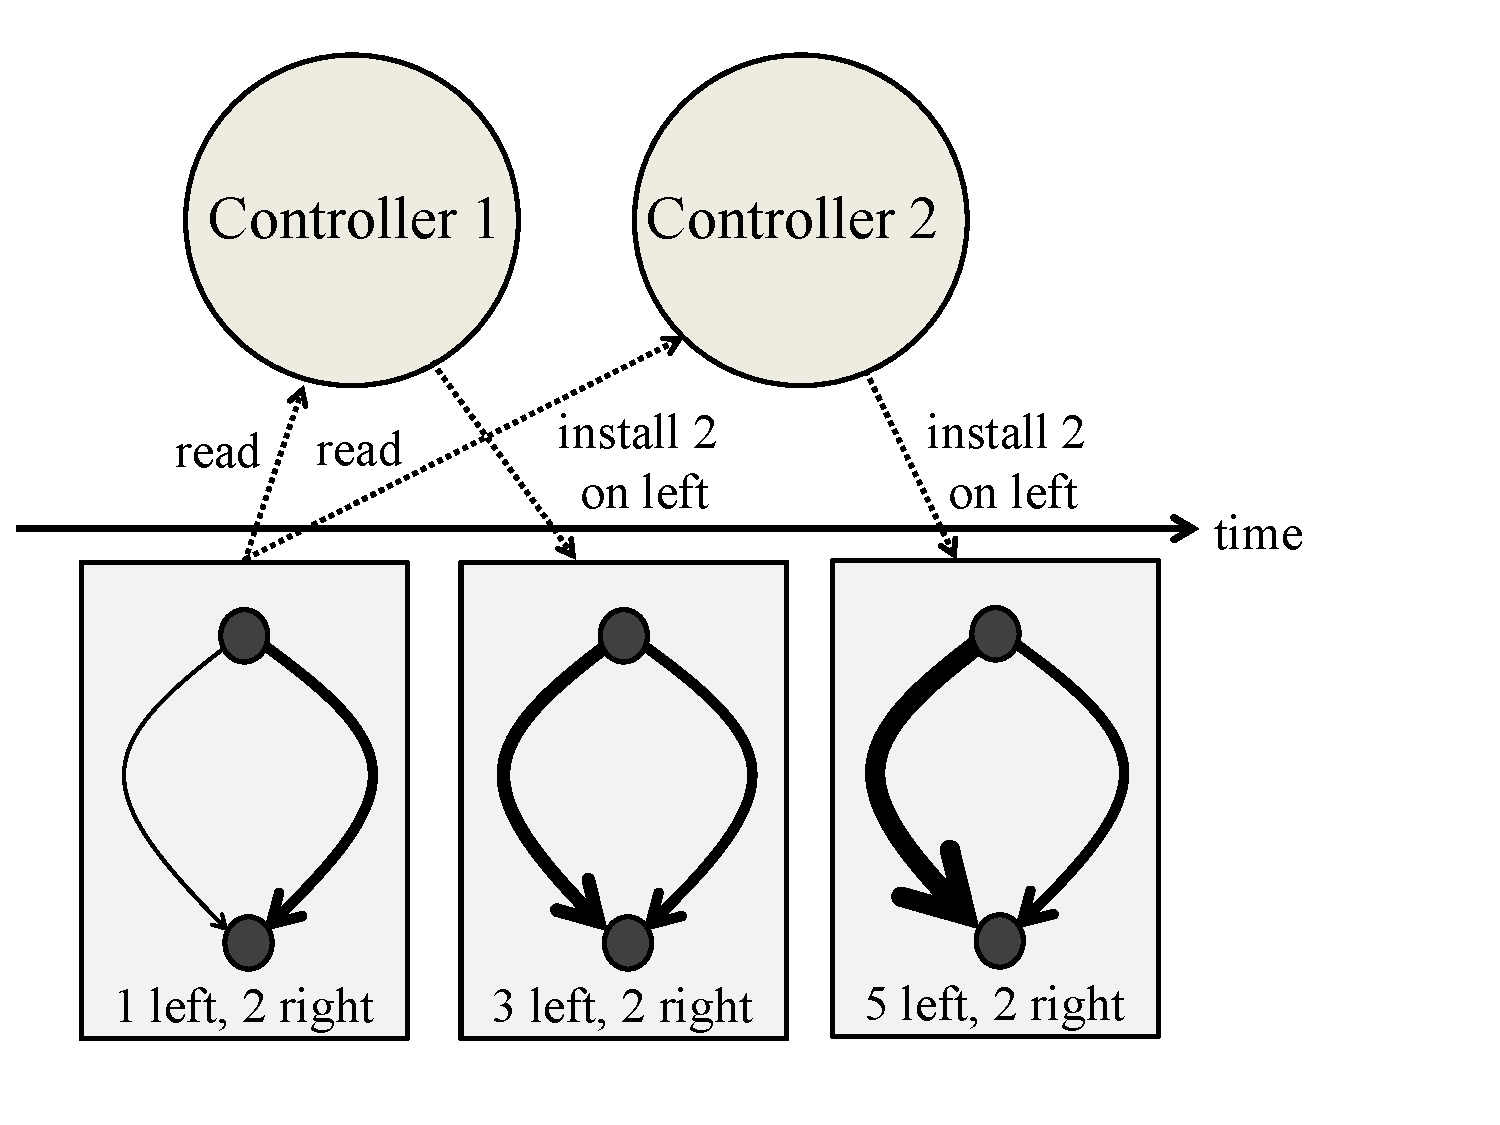
\includegraphics[width=.56\columnwidth]{loadbal-1.pdf}~\hspace{-.7cm}~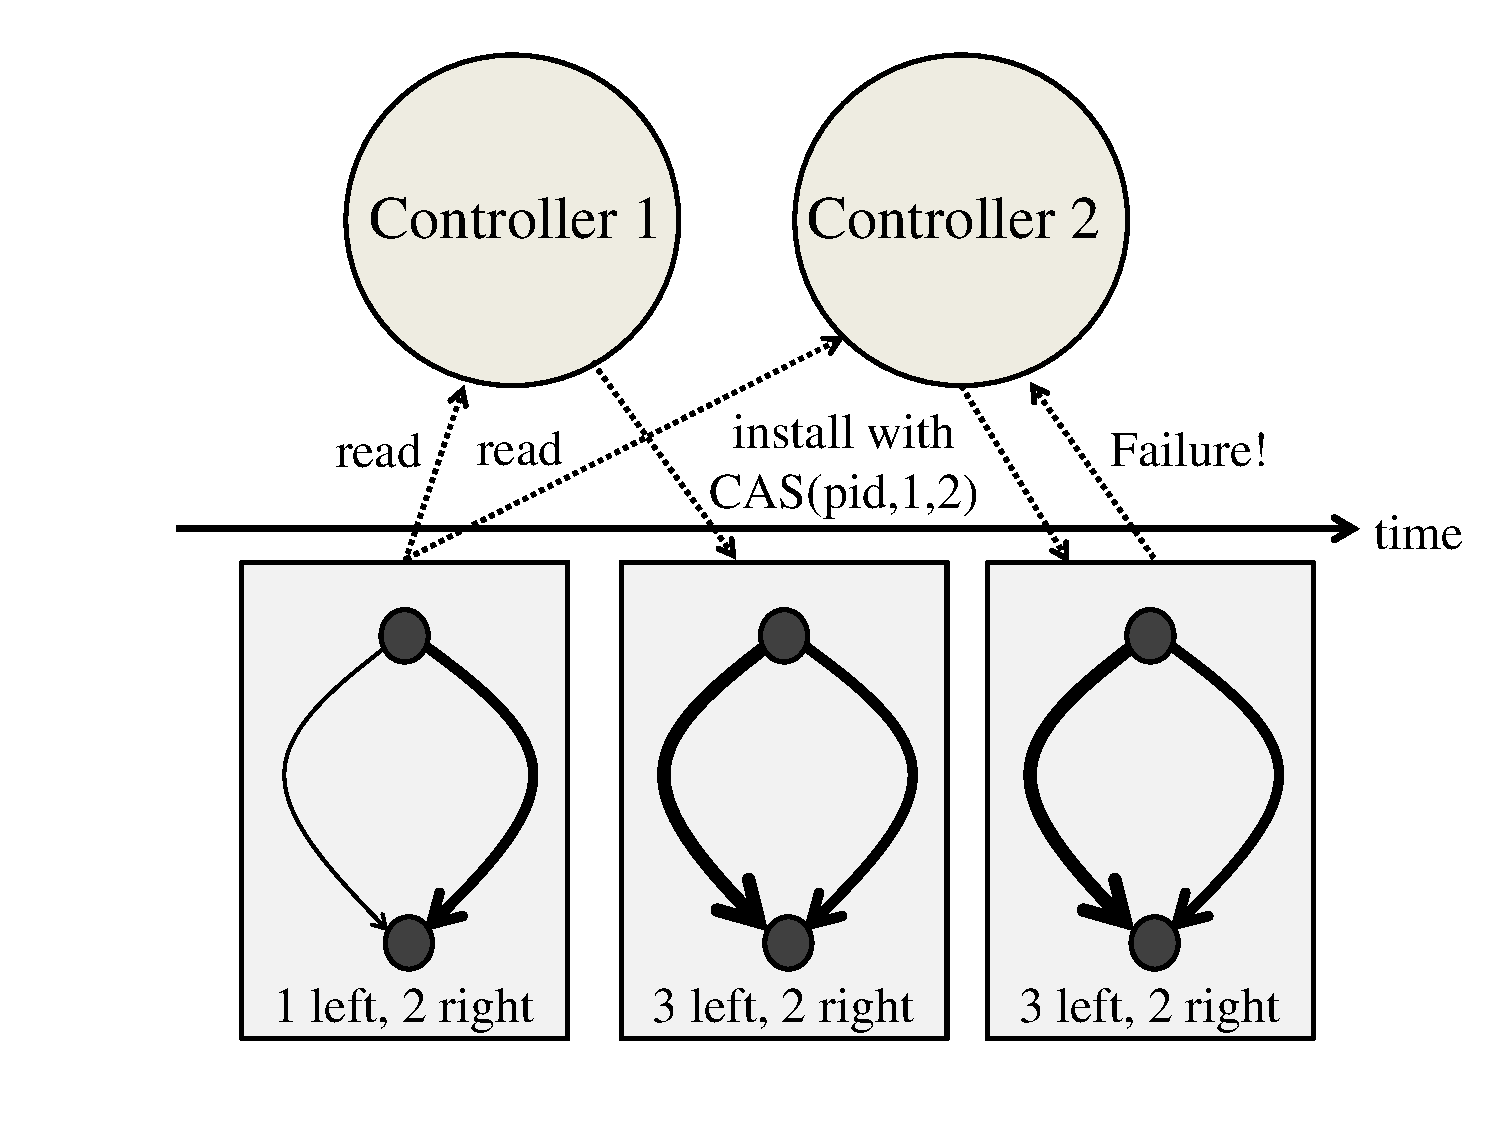
\includegraphics[width=.56\columnwidth]{loadbal-2.pdf}\\
\caption{\small \emph{Left:} Without synchronization, the two controllers naturally choose to
install their flows on the left link, which results in an undesirable
unbalanced state.
 \emph{Right:}
 With synchronization, i.e., by bundling the flow installation with a Compare-and-Set (CAS) primitive
 depending on the policy id (\emph{\pid}), this problem is avoided.}\label{fig:CAS-example}
\end{figure}

\section{In-Band Synchronization}\label{sec:main}

%[[PK how do we know ``minimal''?
In order to synchronize controllers, 
we propose to use a part of the configuration space of the data-plane
switch for storing  a 
%minimal
``meta-data'', containing information
on contention and conflicts between
concurrently installed policy updates. 
%]]
Controllers can read and modify
this meta-data by applying synchronization primitives.
In the following section, we
describe how this space can be organized and consistently maintained
by multiple controllers despite of concurrency and conflicts.


\vspace{1mm}
\noindent\textbf{Configuration space.}
%
We distinguish two parts of the configuration space of a switch:
the ``normal'' configuration which determines the network policy and
is used to process the data-plane traffic (e.g., forwarding rules),
and the \emph{meta-configuration} that contains information used by the
controllers to synchronize their actions.
Flow entries in the meta-configuration can be referred to as shared
memory locations, each provided with a distinct \emph{address}.

The meta-configuration is implemented as a set of flow entries
designed in a way that it does not affect the processing of data plane
traffic. 
We will later discuss later how this can be achieved, for example in 
today's OpenFlow.

%One way to achieve this, for example, is to set a low priority to
%the meta flow entries and ensure that the regular flow entries
%maintain higher priority levels. We will discuss other options later
%in the context of OpenFlow.


%\petr{How to make sure that traffic is not affected by the ``meta'' part?}
\vspace{1mm}
\noindent\textbf{Synchronization.}
 %
We provide the controllers with the ability to execute
sequences of \emph{operations} on the
switch configuration in an \emph{atomic} (transactional) or \emph{non-atomic} mode.
In the atomic mode, either \emph{all} operations in the sequence, henceforth simply
called \emph{transaction},
should be executed, or none (the transaction is rejected).
In the non-atomic mode, no atomicity guarantees are provided.

We introduce two constructs
%$\textbf{bundle}\{\;\ldots\;\}\rightarrow res$ to refer to represent a
$\exec\{op_1,\;\ldots\;op_k\}$ and $\execatomic\{op_1,\;\ldots\;op_k\}$
which perform a sequence of commands $op_1,\ldots,op_k$ in
a regular and atomic way, respectively.
In particular, the construct $\execatomic\{op_1,\;\ldots\;op_k\}$  
returns $\ack$ if and only if all commands in the sequence are performed successfully; otherwise
$\error(\xid,\ecode)$ is returned, providing
the identifier of the first command in the sequence that failed
together with the corresponding error code.


\vspace{1mm}
\noindent\textbf{Synchronization primitives.}
%
We aim to enforce a consistent use of  \emph{policy identifiers},
an important notion in consistent policy updates~\cite{network-update,stn}.
Intuitively, a controller should
equip each to-be-installed policy with a distinct
identifier,
%[[PK do not want to say ``unique'': we also need to motivate claimer-id]]
and the installation should succeed only if the identifier of the
currently installed policy has not changed since the last time the
controller read it.

Therefore, we provide the following (transactional) operations.
A $\textit{write}(\addr,k)$ operation sets the content at memory location
$\addr$ to $k$.
A $\textit{\compare}(\addr,k)$ operation \emph{aborts} the transaction
if and only if the content at
$\addr$ is \emph{not} $k$.
Intuitively, by combining compare and write with a set of regular
switch update commands (e.g., FlowMod in OpenFlow) 
in a transaction  we can make sure that the
configuration is changed and the current policy identifier is updated
only if the check operation \emph{succeeds} (i.e., does not abort).

To make sure that policy identifiers do not grow without bound~\cite{stn}, we
also provide an \emph{id-claimer} object.
The object implements a weak type
of locking by allowing a controller to claim a \emph{resource identifier} in a
given set, release an identifier,  and check if a given identifier
is currently claimed by any controller.
More precisely, the id-claimer object exports three operations \emph{claim},
\emph{unclaim} and \emph{\claimcheck} with the following sequential
semantics:

\begin{itemize}
\item With $\textit{claim}(k)$,
%  $k\in\Nat$,
a controller %$i\in[N]$
\emph{claims}  identifier $k$.

\item With $\textit{unclaim}(k)$, %$k\in\Nat$,
the controller %$i\in[N]$
  \emph{unclaims} identifier $k$.
An identifier $k$ is called \emph{claimed} at a given point of an
execution if there is a controller that has performed $\textit{claim}(k)$
but has not yet performed  $\textit{unclaim}(k)$.

\item With $\textit{\claimcheck}(k)$, the controller checks if $k$ is
  currently claimed by any controller, and if so, the current transaction is
  aborted.

\end{itemize}



\section{Case Study: OpenFlow}\label{sec:background}
%\petr{ the 1st sentence does not belong here}\liron{I think it serves as a motivation for the section, but it fines by me to remove it}

As a case study, in this section, we show how to implement
our transactional approach using today's standard SDN protocol,
 OpenFlow. 

\subsection{Background}

The configuration of an OpenFlow switch is a set of
\emph{rules}.
A rule is essentially a \emph{match-action} pair:
the match part of a rule identifies the space of packet headers that are
subject to the rule (e.g., all packets to a specific destination) and
the action part identifies how the switch should process the matched
packets (e.g., forward them to a specific port).
More precisely, the match part of a rule is
a ternary pattern over packet \emph{header} fields.
The pattern is represented as a \emph{value} and a \emph{mask}.
%\liron{we need to discuss about this, I am not sure this description is accurate.}
In the mask, certain header fields, e.g., TCP or UDP port numbers or destination and source
addresses, can be \emph{wildcarded}, stipulating that their content does
not affect the match.
Certain fields, such as \emph{ipv4\_src}, \emph{ipv4\_dst}, \emph{metadata}, can be arbitrarily
bitmasked.
In our implementations, we are going to use bitmasking of the \emph{metadata}
field for performing conditional operations based on  its content.
%[[PK put the example back in response of review 2
For example, \texttt{ipv4\_src=10.1.14.0/ff.ff.ff.f0} matches all packets
with source IP addresses in the range \texttt{10.1.14.0}--\texttt{10.1.14.15}.
%]]

A \emph{configuration} of an OpenFlow switch is represented as a
collection of \emph{flow tables}.
A flow table is a set of \emph{flow entries}, each containing a rule,
with a match, an action, and a \emph{priority} level, and flow entries
are ordered according to their priorities.
In the simplest setting, a switch maintains one flow table (table 0).
A data-fplane packet arriving at a switch is first checked against
the rule with the highest priority and in table $0$.
If the header of the packet fits the match fields of that rule,
a default \emph{instruction} associates the packet with the corresponding action.
Otherwise, the packet is checked against flow  entries with lower
priorities, and if no matching rule is found, the packet is dropped.

%[[PK move pipelining to the discussion?
\hide{
Furthermore, an OpenFlow switch may maintain multiple flow tables
forming a \emph{pipeline}.
Data-plane packets are checked against flow entries in the pipelined
tables to determine the set of actions the switch should perform on the packet.
A data-plane packet arriving at a switch is first checked against
the rule with the highest priority and in table $0$.
If the header of the packet fits the match fields of that rule,
a default \emph{instruction} associates the packet the corresponding action.
Otherwise, the packet is checked against flow  entries with lower
priorities.
Specific instructions can be used to define
additional tables to be visited (\textit{goto} instructions), to
modify the set of actions associated with the packet (by adding,
deleting or modifying actions), or immediately apply some actions in the action set.
During the traversal of the flow tables, the packet can also be equipped with \emph{meta-tags} to
transfer temporary information between tables.
The meta-data field is part of the header that can be
inserted or removed from a packet via \emph{push} and \emph{pop}
actions.

The actions associated with the packet are performed at the end of the pipeline.
If no rule matches the packet, the packet is dropped.
\petr{do we need the discussion of multiple tables/pipelining here? I still find it
  very confusing}



\liron{we should explain that: every packet is associated with an
  action set. This set is empty at the beginning and is changed
  according to the flow table matches. Each match is asociated with
  instructions that can add or modify actions in the action set and
  also to apply (now) all actions in the action set. By default action
  set is applied at the end of the pipeline.}
}

%\liron{I think that maybe the rest of this section should be explained by the following subsections, providing in depth description of the OpenFlow features.}
%\liron{Another direction is to have a simplified explenation as now and to refference spesific sections of the standard in side our paper.}
\vspace{1mm}
\noindent\textbf{Interaction between the planes: FlowMod commands.}
The flow tables installed on the switches across the data plane
determine the network \emph{policy}.
Controllers can change the policy by sending
control messages containing \emph{FlowMod commands}.
In a nutshell, a \emph{FlowMod} command either specifies a new flow entry or
a modification to an existing flow entry.
%
%
%[[PK already said
%A flow entry consists of: (1)~a match
%field
%(a value and a mask), (2)~a set of actions, and (3)~a priority.
%]]
%
%
A FlowMod command can either add a flow entry or delete a flow entry.
The standard processing of a FlowMod $\add$ command received by a switch is
as follows.
If the switch already maintains a flow entry with \emph{exactly} the
same match and priority level, then the new flow entry will simply \emph{replace} it.
Otherwise, the flow entry will be installed in addition to existing
ones.
A $\dele$ command simply removes an existing flow entry with the same
match and priority,  or does nothing if such an entry is not present.
%Stefan: alternatively could also delete an entry by using the cookie field

%\petr{Is this correct?}

%but will be installed
%\emph{in addition} to existing entries if they only
%partially overlap (or define flowspace subsets or supersets).

%If rules with overlapping but not identical match fields have the same priority,
%inconsistencies can arise, since there is no clearly specified action
%that should be applied to a packet matching the two entries.
%[[PK shortened
In order to avoid inconsistencies caused by different rules with
overlapping match fields, a \emph{FlowMod} command can be equipped with 
the $\checko$ flag which will be instrumental
in implementing our synchronization abstractions:
if the switch maintains a flow entry with an overlapping but not
identical match part with the same priority, then
the \emph{FlowMod} command will fail.
%The $\checko$ flag in a \emph{FlowMod} command helps resolving simple
%conflicts between controllers, and will be instrumental
%in implementing our synchronization abstractions.
%]]

%[[PK not sure this is the right place
%implement synchronization objects which form
%the basis of our transactional interface.
%]]
We will use the following notation to create a \emph{FlowMod} message:
$\FlowMod(\match, op, \action, \flags)$, where
%$\match$ denotes the match,
$op$ is $\add$ or $\dele$, and $\flags$ are used, e.g.,  to activate the $\checko$
feature.
For simplicity, we omit other standard parameters, assuming them to carry
default values.
%A standard \emph{FlowMod} message (and also the flow entries) may specify
%more parameters, which are however irrelevant for our implementation, and we suggest to
%use the default values.

To read the current configuration of a switch (the existing flow entries), the controller should send
the OpenFlow \emph{add flow monitor} command with the \textsf{ofpt\_initial} optional flag.
In this paper, we write \textbf{read-state} for sending
this message, receiving a response, and returning the received configuration.
\petr{Is it atomic? Should we say that the command returns a ``snapshot'' of the
  configuration?}

\vspace{1mm}
\noindent\textbf{Bundling.}
%
Another important feature in OpenFlow is \emph{bundling}. %(as of OpenFlow version 1.4). \stefan{liron, is that correct?}
A controller can send multiple $\FlowMod$ commands  equipped with
the same \emph{bundle identifier}.
These commands are buffered temporarily by
the switch until a \emph{bundle commit} message is received from the
controller.
The bundled commands are then performed with \emph{all-or-nothing semantics}:
either all of them are performed, or none of them is.
In particular, if a configuration request contained in one of the bundled commands cannot
be applied (e.g., the command is rejected because of the set
$\checko$ flag and a conflicting flow entry), all  other commands in
the bundle are rejected and an error
message is sent to the controller that issued them.
%If multiple \emph{FlowMod} messages with the $\checko$ flag are sent as a single bundle,
The error message contains $\xid$, the identifier of the first failed command in the
bundle, and $\ecode$, the identifier of the failure.

A bundle begins with a  \texttt{ofpt\_bundle\_control} message of type
\texttt{ofpbct\_open\_request} (creating the bundle), wraps
each of its \emph{FlowMod} command in a message
\texttt{ofpt\_bundle\_add\_message} equipped with the \emph{bundle
  identifier}, and ends with a \texttt{ofpt\_bundle\_control} message of
type \texttt{ofpbct\_commit\_request} (committing the bundle).

%[[PK too detailed and not very clear
%Concretely, when the commit fails, the switch must generate an error message corresponding to the
%message that could not be applied. The error message must use the identifier (\emph{xid}) of the offending message,
%the error data field corresponding to that message and the error code corresponding to the failure. If
%multiple messages are generating errors, the switch may return only the first error found or generate
%multiple error messages for the same bundle.
%]]


%Again, the bundle always returns a binary result: \emph{error} ($\bot$) or \emph{success} ($\top$).

%When properly configured,
The bundle execution is \emph{controller-atomic}
in the sense that all controllers can only observe switch
configurations \emph{before} or \emph{after} the
bundle commands are executed.
We set the flag \texttt{ofpbf\_atomic},
making bundles \emph{packet-atomic},
in the sense that every data-plane packet is processed by a configuration
before or after the bundle, and not by a configuration resulting from
an incomplete bundle execution.
We also set the flag \texttt{ofpbf\_ordered},  to make sure that the
bundle commands are executed in the order they were added to the
bundle, thereby respecting dependencies between bundle commands.

\subsection{Implementation} 

At first sight, it may seem that bundling \emph{FlowMod} commands with  the $\checko$
flag already provides a useful synchronization mechanism.
Indeed, its ``mini-transaction'' nature allows a controller
to install multiple flow entries in an atomic way.
However, as is,
bundling has important limitations. %, as we will argue in the following.

First, %if employed without any additional features,
except for some limited constraint types (such as
overlapping flow spaces or insufficient free space),
the bundle construct \emph{per se} 
does not provide any means to modify the switch configuration
based on application-specific conditions.
%[[PK overlapping flow spaces also depend on the switch configuration...
%, which depend on the
%current configuration.
%]]
But, as we have seen in our load-balancing
example, supporting such conditions 
%under which configuration updates should or should not take place, 
might be essential.
Second, it is sometimes desirable to react to conflicts in smarter ways than
by simply aborting an operation, e.g., by providing \emph{conditional modifications}.

%[[PK Why ``nevertheless''? 
%Nevertheless, 
We now show that the OpenFlow match-action paradigm 
can be used  to realize a transactional synchronization abstraction
with the desired functionality. 
%Concretely, the OpenFlow match-action paradigm can be used
%to implement a key-value store.
%]]
The 
%OpenFlow 
meta-configuration can be realized using low-priority rules.
Alternatively, we can leverage the possibility to maintain multiple
flow tables at an OpenFlow switch, and use a separate flow table for
the meta-configuration,  making sure that the
\emph{pipelining} mechanism will never involve this
flow table.

Recall that a transaction consists of a sequence of operations,
each of which can either be a regular FlowMod command or a synchronization
primitive, which, as we
show below, translates into a sequence of FlowMod commands operating on the
switch meta-configuration.

The implementation of $\exec\{op_1,\ldots,op_k\}$ and
$\execatomic\{op_1,\ldots,op_k\}$ constructs
invoked by a control application is simple.
First we translate  $op_1,\ldots,op_k$ into a sequence of FlowMod
commands. If $op_i$ is already a FlowMod command, the translation is
trivial. If $op_i$ is a synchronization primitive, we employ
Algorithm~\ref{alg:claim} for $\textit{claim}$,
Algorithm~\ref{alg:check} for $\textit{checkclaim}$,
Algorithm~\ref{alg:unclaim}
for $\textit{unclaim}$,
Algorithm~\ref{alg:write} for $\textit{write}$ and
Algorithm~\ref{alg:compare} for $\textit{compare}$.

To implement  $\exec\{op_1,\ldots,op_k\}$, we simply send the commands in
the resulting sequence, one by one, to the switch.
%
To implement  $\execatomic\{op_1,\ldots,op_k\}$, we
additionally create a bundle, wrap each of the resulting commands in a
bundle message with the corresponding bundle identifier, and complete it
with a bundle commit message.
Then we wait until the
corresponding responses are received.
If an error message is returned,
it is forwarded to the control application,
otherwise it is $\ack$ed.

We now describe Algorithms~\ref{alg:claim}-\ref{alg:compare} in more
detail.
Each of the operations generates one or two FlowMod commands.
The \textit{match} part in these commands specifies only the $64$bit meta-data
field in the header space, leaving the remaining fields at default
values.
In defining the value and the mask,
% of the math part,
we
use the notation $a\concat b$ to represent a concatenation of two
 integers $a$ and $b$: $a\concat b := (a<<s)+b$, where $s$ is the size of $b$ in bits.
We also write \texttt{$\ones{s}$} (\texttt{$\zeros{s}$}) for  a $s$ bit 
string of $1$'s ($0$'s).
%
The action part in these commands is defined as an integer, which in
practice can be implemented by a \emph{set meta-data} instruction where the written value is that integer.


\hide{
%[[PK too lengthy, partially said before
To simplify the presentation we set the FlowMod command field values with integers, according to the following guidelines:
\begin{itemize}

\item {\bf  Flag:} we often use the $\checko$ optional flag value to make the command execution dependent on switch state. In other cases, when the flag value remains zero, we omit the assignment.

\item {\bf  Match:} we consider the match part of an entry to be a ternary string of bounded length, represented by binary strings (integers) named value and mask. In general, the match can be applied to any set of supported packet header fields. In our implementation, the $64$bit meta-data field alone is sufficient. We sometimes use the concatenation of two integers, denoted by $a\concat b$, to form one match value or mask, where $a\concat b := (a<<s)+b$ and $s$ is the size of $b$ in bits.

\item {\bf Action:} we consider the action part of an entry to be an integer, which in practice can be implemented by a \emph{set meta-data} instruction where the written value is that integer.

\end{itemize}

In addition we use "op" as shortened form to a field that indicates whether the command should $\add$ or $\dele$ the specified flow entry. This corresponds to the FlowMod field named "command" which can receive values \textt{ofpfc\_add} and \texttt{ofpfc\_delete}.
%]]
}

\vspace{1mm}
\noindent\textbf{The id-claimer.}
%
In Algorithms~\ref{alg:claim}-\ref{alg:unclaim},
the match part of the constructed commands represents a concatenation
of claimed identifier with a distinct $16$bit controller identifier.
%In addition, every controller uses a unique mask part of the match
%defined as a distinct $32$bit controller identifier concatenated with
%\texttt{1$\ldots$1}.
This allows multiple controllers to claim the same identifier without
overriding existing flow entries (Algorithm~\ref{alg:claim}).
%
For example, for any two resource identifiers $x_1$ and $x_2$ and controller identifiers $c_1\neq c_2$,
the match patterns
%$m_1=(c_1\concat x_1, \ones{48})$ and $ m_2=(c_2\concat x_2, \ones{48})$ 
$m_1=(*^{16}\concat c_1\concat x_1)$ and $ m_2=(*^{16}\concat c_2\concat x_2)$ 
are distinct,
even if $x_1=x_2$.
Therefore, they can both be used to claim and unclaim identifiers without affecting each other.
In order to distinguish between claim entries and other policy
entries, %[[PK ``some magic value'' sounds magic... 
we set the action part of the entries storing claimed ids to
be a unique designated value, $\claimmagic$.


In order to check if an identifier $x$ is claimed
(Algorithm~\ref{alg:check}), a controller $c$ tries to add
a ``tester'' entry, where the match value field is 
$(c\concat*^{16}\concat x)$  and the flag \texttt{\checko} is set.
Note that the controller identifier is shifted $16$ bits to the left in
the match field, which allows us to ensures that the entry is uniquely
identified, while not conflicting with other entries.  
This attempt inflicts a failure in case another entry with claimed
value $x$ exists. 
If the check succeeds, i.e.,  no entry with claimed value $x$ is
present, the tester entry is deleted.   
%[[PK unnecessary?
%In any case since the check entry contains the controller id, it does not conflict with other check entries and there is no negative impact of delaying the deletion.
%]]
%Considering $m_1$ and $m_2$ from the example above,
%with respective actions $a_1=1$ and $a_2=2$,  they overlap
%with different actions iff $x_1=x_2$. Therefore, if $m_1$ is used in the \claimcheck after $m_2$ was used in the claim operation,
%a conflict is detected iff $x_1=x_2$, as desired.

%[[PK too wordy?
%Note that in order to save space, when checking for claims, also the deletion of the added tester flow entry is included,
%which however has no effect on claims and checks of other controllers; hence, the deletion command does not
%have to be sent as part of a bundle. Therefore, the \texttt{\claimcheck} operation is atomic by nature,
%similar to the \texttt{claim} and \texttt{unclaim} operations, and is
%implemented as essentially one command.
Note that the tester rule has no effect on claims and checks of other
controllers. Hence the add and delete commands do not have to be
executed atomically (e.g., within a bundle): the \texttt{\claimcheck}
operation ``takes effect'' at the moment it attempts to add the tester entry.   
%Hence, the deletion command does not
%have to be sent as part of a bundle. Therefore, the \texttt{\claimcheck} operation is atomic by nature,
%similar to the \texttt{claim} and \texttt{unclaim} operations, and is
%implemented as essentially one command.
%]]

%[[PK isn't it obvious?
By employing the \textbf{read-state} command, we may easily implement
an additional operation that returns all currently claimed ids: it is
sufficient to go over the rules matching every controller identifier
carrying action $\claimmagic$.
%]]
%[[PK
%In order to distinguish between claim entries and other policy
%entries, returned by  \textbf{read-state},
%%[[PK ``some magic value'' sounds magic... 
%we set the action part to
%be a unique designated value, $\claimmagic$.
%%]]
%]]

{\scriptsize

\begin{algorithm}[t]
    \caption{$\textit{claim}(x)$}
    \label{alg:claim}
    \begin{algorithmic}[1]
    \Require \emph{self} as the calling controller id.
%    \Ensure
    		\State $\textit{value} \gets \zeros{16}\concat self\concat x$
    		\State $\textit{mask} \gets \zeros{16}\concat\ones{16}\concat\ones{32}$
	    	\State $\textit{match} \gets (\textit{value},\textit{mask})$
    		%\State $cookie \gets x\concat self$
    		\State $\textit{action} \gets \claimmagic$
    		%\State $\textit{flag} \gets 0$
    		\State $\textit{cmd}\gets \textit{FlowMod}(match, op = \add, \textit{action}) $
			\Return $\textit{cmd}$
    \end{algorithmic}
\end{algorithm}

\begin{algorithm}[t]
    \caption{$\textit{\claimcheck}(x)$}
    \label{alg:check}
    \begin{algorithmic}[1]
    \Require \emph{self} as the calling controller identifier.
%    \Ensure
    		\State $\textit{value} \gets self\concat \ones{16}\concat x$
    		\State $\textit{mask} \gets \ones{16}\concat \zeros{16}\concat \ones{32}$
    		\State $\textit{match} \gets (value,mask)$
    		%\State $cookie \gets x\concat self$
    		\State $\textit{action} \gets \claimmagic$
    		\State $\textit{flag} \gets \texttt{ofpff\_\checko}$
    		\State $\textit{cmd1}\gets \textit{FlowMod}(\textit{match}, op = \add, \textit{flag}, \textit{action}) $
    		\State $\textit{cmd2}\gets \textit{FlowMod}(\textit{match}, op = \dele) $
			\Return $\textit{cmd1}$,$\textit{cmd2}$
    \end{algorithmic}
\end{algorithm}

\begin{algorithm}[t]
    \caption{$\textit{unclaim}(x)$}
    \label{alg:unclaim}
    \begin{algorithmic}[1]
    \Require \emph{self} as the calling controller id.
%    \Ensure
    		\State $\textit{value} \gets \zeros{16}\concat self\concat x$
    		\State $\textit{mask} \gets \zeros{16}\concat\ones{16}\concat\ones{32}$
    		%\State $cookie \gets x\concat self$
    		\State $\textit{match} \gets (\textit{value},\textit{mask})$
    		\State $\textit{cmd}\gets \textit{FlowMod}(\textit{match}, op=\dele) $
    	
			
			\Return $cmd$
    \end{algorithmic}
\end{algorithm}
}

\vspace{1mm}
\noindent\textbf{Write and compare.}
The memory \memwrite and \compare
 operations are implemented using similar techniques.
To write a value $k$ in a memory address $\addr$ (Algorithm~\ref{alg:write}), a new flow entry is
added, in which the value part of the match field contains $\addr$ and
the mask part contains $k$. 
Therefore, the effective match string od the entry 
 is $k'\concat \addr$, where $k'$ is result os replacing every zero bit in $k$ with a wildcard ($*$).
  In order to rewrite a memory location, the old entry needs to be deleted and a new one need to be added atomically.
  %Values written to the same address will replace one another,
%following the command definition to replace the old flow entry with a new one in case they
%share the same match parts.
Similarly to claim entries, we set the action to a magic value,
$\memmagic$, in order to distinguish them from policy entries.
%[[PK not needed?
%returned by \textbf{read-state}.
%]]

To check whether a value $k$ is written at a given
address $\addr$ (Algorithm ~\ref{alg:compare}),
a controller tries to add a new entry the same way as in the \memwrite operation,
but additionally setting the \texttt{\checko} flag. 
If a different value $k'$ is currently written, 
%our action differs from the existing entry, but 
the entry inflicts a failure, as it overlaps but does not coincide
with the existing entry.
Indeed, the value parts of the two entries are identical, but the
masks differ.
% \liron{(different mixtures of ones and wildcards in the $k'$ part)},
%thereby inflicting a failure. 
In case the currently written value is $k$, the existing flow entry is replaced
with an identical one.

\liron{Note that comparing an uninitialized address always succeeds and also writes to it the compared value. Initializing required addresses can be safely performed by an a-priori comparison with zero.}
\petr{A bit unclear}

%HERE: we can read state by reading flow monitor => read configuraiton abstraction => state of claimer ID objects list of all claimed identifiers

{\scriptsize

\begin{algorithm}[t]
    \caption{$\textit{write}(\addr,k)$}
    \label{alg:write}
    \begin{algorithmic}[1]
    %\Require  id $i$.
%    \Ensure
    		\State $value \gets \ones{32}\concat\addr$
    		\State $mask \gets  \zeros{32}\concat\ones{32}$
    		\State $match \gets (value,mask)$
    		\State $\textit{cmd1}\gets \textit{FlowMod}(\textit{match}, op = \dele) $
    		
  		   \State $value \gets \ones{32}\concat\addr$
  		   \State $mask \gets  k\concat\ones{32}$
  		   \State $match \gets (value,mask)$
 		    		%\State $cookie \gets x\concat self$
 		   \State $action \gets \memmagic$
 		   %\State $flag \gets 0$
		   \State $\textit{cmd2}\gets \textit{FlowMod}(\textit{match}, op = \add,  \textit{action}) $
		    		
			\Return $\textit{cmd1}$,$\textit{cmd2}$
    \end{algorithmic}
\end{algorithm}

\begin{algorithm}[t]
    \caption{$\textit{\compare}(\addr,k)$}
    \label{alg:compare}
    \begin{algorithmic}[1]
    %\Require  id $i$.
%    \Ensure
    		\State $value \gets \ones{32}\concat\addr$
    		\State $mask \gets  k\concat\ones{32}$
    		\State $match \gets (value,mask)$
    		%\State $cookie \gets x\concat self$
    		\State $action \gets \memmagic$
    		\State $flag \gets \texttt{ofpff\_\checko}$
    		\State $cmd\gets \emph{FlowMod}(match, op = \add, flag, action) $
			\Return $cmd$
    \end{algorithmic}
\end{algorithm}
}


\section{Applications}\label{sec:apps}

Our synchronization primitives can be used to 
implement powerful synchronization primitives such at
\emph{compare-and-set} (CAS).
When executed within a transaction, a $\cas(\addr,\textit{old},\textit{new})$ operation 
on a memory location $\addr$
checks if the content of $\addr$ is $\textit{old}$ and if so,
replaces it with $\textit{new}$ %and returns $\true$ 
(the CAS \emph{succeeds}), otherwise it 
%returns $\false$ 
causes an abort of the invoking transaction
(the CAS \emph{fails}).
It is straightforward to implement the CAS operation by executing
$\textit{\compare}(\addr, old)$ followed by $\textit{\memwrite}(\addr,
new)$ within the {\execatomic} construct.

Let us now revisit our load-balancing application
discussed in Section~\ref{sec:motivation}.
A simple strategy to balance load in our 2-link example
 (Figure~\ref{fig:CAS-example}) fails in the presence of
multiple controllers, even if 
bundling and $\checko$ features are used:
the flows are defined over ``independent'' 
flow spaces. 

%[[PK ``render concurrent''? we already discuss a concurrent setting...
%As we show in the following, our mechanisms can be used 
%to render such algorithms concurrent.
Using CAS, we can implement a
generic template 
for concurrent policy composition via a user-specific
$\textsc{\ufunc}()$ function~\cite{stn}.
This can be, for example, a specific load-balancing
function $\textsc{lb\_update}$, %\petr{Did we talk about this function before?}
which, when applied atomically, excludes the pathological scenario described in 
Figure~\ref{fig:CAS-example}. 
We use CAS to exactly achieve this atomicity.
% if we put
%the policy update in our transactional $\execatomic$ construct together
% with a \emph{Compare-and-Set} (CAS) operation on the policy identifier.

Let us consider a simple policy update protocol that
allows a set of  controllers to concurrently update switch policies, i.e., sets of
%[[PK policies have been defined in Background]]
effective flow entries, under the
condition that these rules can be \emph{composed} with the currently installed
policy.
Algorithm~\ref{alg:simple-update} uses the bundle feature to update
the switch configuration, where the configuration contains both the
policy and a meta-configuration memory address $\paddr$ that holds the \emph{policy identifier (\pid)} .
In the algorithm, the controller first reads the currently installed
policy together with its {\pid},  applies the
$\textsc{\ufunc}()$ function to the current policy which results in a
set of update FlowMod commands and then tries to apply them
atomically together with a CAS operation on $\paddr$ replacing $\pid$
with $\pid+1$.
The latter ensures that if, concurrently, a new policy (with a different identifier) has been installed, the update
fails and takes no effect.
Algorithm~\ref{alg:simple-update} can therefore also be used
to render a na\"ive, single-controller load-balancing algorithm
consistent, without any modifications in the update function.

% \liron{the term composition doesn't make sense now with the new user update function... }

%\liron{we can explain how a normal controller code can be instrumented to use our paradigm}
%\petr{did not get the comment}

%[[PK clear from the algorithm?]]
% and use them in order to make sure that the new policy, with id
%$\pid+1$, replaces the (what considered as) current policy, with id
%$\pid$.
%Considering the policies identifiers, we send the policy update
%commands as part of a bundle that also tries to perform
%$CAS(\pid,\pid+1)$, thereby insuring that the commands are
%performed iff the current policy is still there and preventing other
%controllers to replace the new policy with another without observing it.

%\petr{what does it mean for an update function to be ``unsafe''?}

%For brevity, we omit explicitly putting the $\textbf{bundle}\{...\}$ construct
%around each of the transactional operation used in the algorithm.
%Indeed, since \textit{claim} and \textit{unclaim} operations cannot
%cause the corresponding transaction, we can assume that all
%``singleton'' (consisting of one operation only)  transactions
%containing such operations always commit. \liron{I think we can ommit this paragraph entirely - no need for bundle when it is not written}

{\scriptsize
\begin{algorithm}[t]
    \caption{Policy update with only CAS}
    \label{alg:simple-update}
    \begin{algorithmic}[1]
    \Require policy update function \textsc{\ufunc}, policy id address $\paddr$
    \Ensure installed policy is consistent with previous one
 		%\Do
 		\Repeat
 			\State $\pid,\textit{policy}\gets$ \textbf{read-state} %switch configuration}
 			\State $\textit{update\_cmds}\gets \textsc{\ufunc}(policy)$
 			\startTxn
	 			\State $CAS(\paddr,\pid,\pid+1)$,
	 			\State $\textit{update\_cmds}$ %conditioned on $metadata=my\_a$
	 			%\State update policy selector to $my\_a$
 			\endTxn
     		%\State $res \gets $ commit transaction
     	\Until{$\textit{res}=\ack$}
     	%\doWhile{$res=False$}
%   \vspace{3mm}
			\Return $\textit{res}$

    \end{algorithmic}
\end{algorithm}
}



A less trivial Algorithm~\ref{alg:update} adresses the problem of
policy identifiers growing without bound in  
Algorithm~\ref{alg:simple-update} by, additionally, using our id-claimer abstraction.
%to bound the number of used policy identifiers.
Here, the controller first reads the current policy id and 
claims it, which prevents another controller from using the id 
for a different policy (Lines~\ref{update:read-state1}-\ref{update:read-state2}).Then the controller claims the first \emph{unused} id and computes the update commands to be executed (Line~\ref{update:compute}).
Finally, within an atomic transaction (\textbf{\execatomic}), it verifies whether the chosen policy id has not
been claimed and that
the policy has not been concurrently modified, and then updates the
policy.
Unlike Algorithm~\ref{alg:simple-update}, this algorithm is only
\emph{lock-free}, as it allows scenarios in which only one live controller
succeeds in installing its updates. We can easily make it
wait-free by  

\vspace{1mm}
\noindent\textbf{A note on efficiency.}

We observe that our implementations of synchronization primitives
(Algorithms~\ref{alg:claim}-\ref{alg:compare}) 
%is \emph{switch-space efficient}
%in the sense that 
require only a constant number of flow entries per memory address.
The number of used addresses is constant for  
Algorithm~\ref{alg:simple-update} and linear in the number of
controllers for Algorithm~\ref{alg:update}. 
%[[PK not constant: proportional to the number of failures. But this
%is kind of obvious.
%Also, in case of controller failures, at most a constant amount of space is lost.
%]]

\stefan{We also note that while we described our scheme in a simplified
way where numbers continuously increase, it is straight-forward to use a modulo
scheme. While in our case 32-bit numbers are used, 
the flow table width (number of bits which can be matched in parallel)
of modern switches is 40-bits and more.}

 \liron{I think we should say something like: "... of modern switches can get as high as a few hundreds'. }

\petr{The discussion is very confusing. Do we need it?}  



{\scriptsize
\begin{algorithm}[t]
    \caption{Advanced policy update}
    \label{alg:update}
    \begin{algorithmic}[1]
        \Require policy update function \textsc{\ufunc}, policy id address $\paddr$, id space $C$.
    \Ensure installed policy is consistent with previous one
 		%\Do
 		\Repeat
		 	\State $\pid,claims,policy\gets$ \textbf{read-state} \label{update:read-state1} %switch configuration
 			\State $\textbf{execute}\{claim(\pid)\}$
 			\State $\pid 2,\textit{claims},\textit{policy}\gets$ \textbf{read-state} \label{update:read-state2} %switch configuration
 			\If {$\pid\neq \pid 2$}
	 			\State $\textbf{execute} \{\textit{unclaim}(\pid)\}$
 				\State {\bf continue} (\textbf{restart} loop)
 			\EndIf
 			\State $\textit{my\_id}\gets$ choose a number from $C\setminus claims$
 			\State $\textit{update\_cmds}\gets \textsc{\ufunc}(policy)$ \label{update:compute}
 			\startTxn
 				\State $\claimcheck(my\_id)$,
	 			\State $CAS(\paddr, \pid,my\_id)$,
	 			\State $\textit{update\_cmds}$ %conditioned on $metadata=my\_a$
	 			%\State update policy selector to $my\_a$
 			\endTxn
	 		\State $\textbf{execute} \{\textit{unclaim}(\pid)\}$
     		%\State $res \gets $ commit transaction
     	\Until{$res=\ack$}
     	%\doWhile{$res=False$}
%   \vspace{3mm}
			\Return $\textit{res}$

    \end{algorithmic}
\end{algorithm}
}


\section{Proof-of-Concept}

To investigate the feasibility of our approach,
we implemented a proof-of-concept of our algorithms
as a python library which wraps ovs-ofctl, 
a well-known command line tool for monitoring and administering OpenFlow switches. 
The code is publicly available at \url{https://github.com/lironsc/of-sync-lib}.

We experimented with the low-level abstractions as well as the 
transactional policy update algorithm of our proof-of-concept, using
different workloads. 
The tests were conducted using a software switch, Open vSwitch (version 2.4.0) and
a virtual network simulator, Mininet.

For instance, we experimented with a setting where three processes
(controllers) issue thousands of concurrent policy updates
to the switch, 
each update consisting in replacing a single rule with another one.
%[[PK unclear
%When verifying the transactions, 
%]]
We could confirm that 
despite the concurrency, 100 \% of the updates have been
eventually completed.
Of course, due to the concurrency, some transactions also needed to abort
because of conflicts. 
 
While our framework can be used as a synchronization tool itself, we 
currently also work on implementing it as an integral part of existing controllers 
such as Ryu. 
\petr{Did not get the difference between ``itself'' and ``part of
  existing controllers''.} 


\section{Conclusion}\label{sec:conclusion}

%This paper initiated the study of mechanisms which allow distributed controllers
%to synchronize their possibly concurrent actions. 

We believe that our centralized in-band
synchronization approach is natural and attractive, as it avoids the
complexities and limitations of distributed out-of-band agreement protocols, which may 
introduce additional points of potential failures.
Moreover, the switch is the element implementing the controller policies anyway.
The mechanisms presented in this paper are simple and can be implemented using the \emph{standard OpenFlow}
protocol: they do not require any protocol/hardware extensions as postulated in recent literature~\cite{stn,netpaxos}.
Our work may hence also contribute to the ongoing discussion of what can be implemented
in-band in today's OpenFlow protocol~\cite{reclaim},
as well as to useful high-level concurrency objects and
language abstractions~\cite{pyretic}.
In general, we see our paper as a first step, and more
work is required to investigate and compare useful
in-band synchronization abstractions, also in terms of performance.

{
%\begin{footnotesize}
\bibliographystyle{abbrv}
\bibliography{references}  % main.bib is the name of the Bibliography in this case
%\end{footnotesize}
}


\end{document}
